
\section*{Appendix \hypertarget{AppA:Figures}{A}: Figures} \label{App:Figures}

\subsection*{\hypertarget{AppA1:Figures:Excludedc}{A1} Excluded consumer data sets}\label{AppA1:Figures:Excludedc}

\begin{centering}
\begin{figure}[!htbp]
        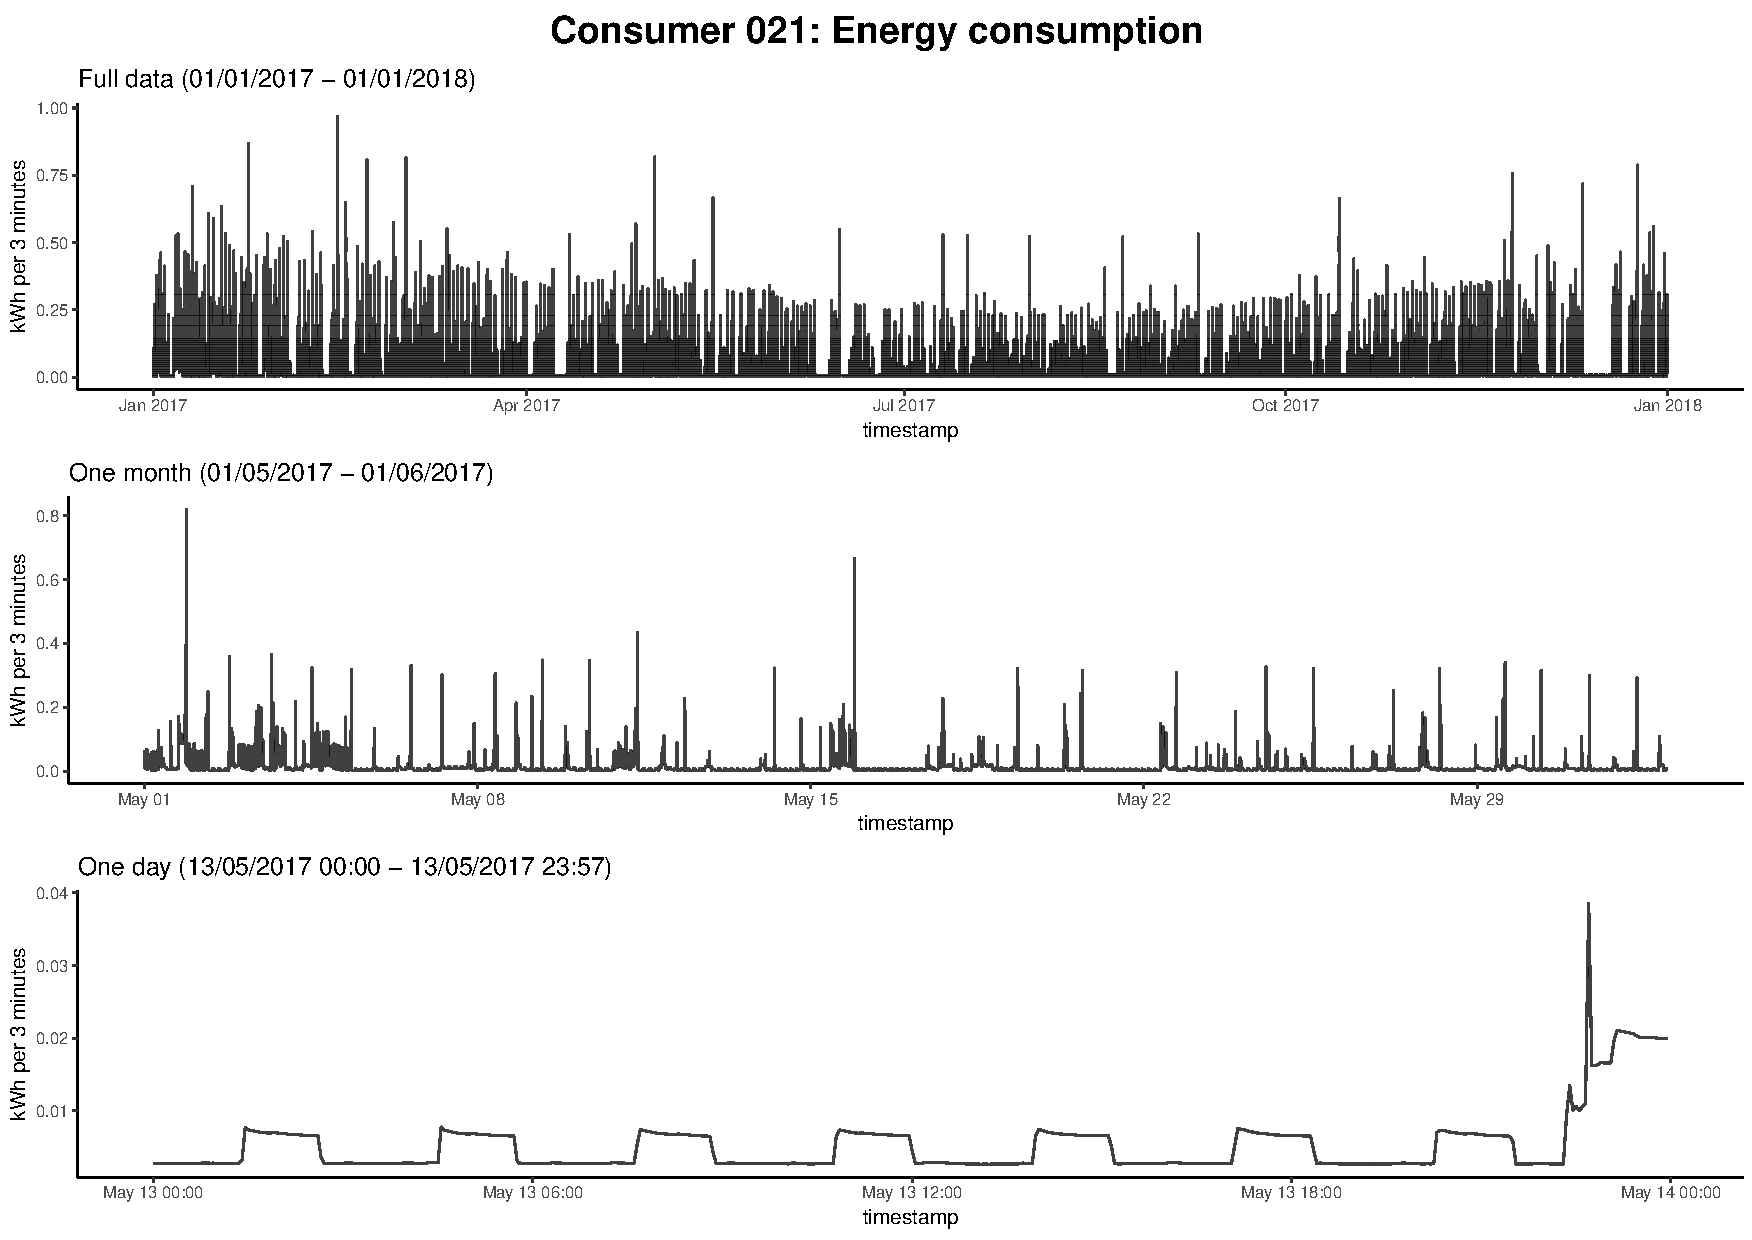
\includegraphics[width=\textwidth-0.85cm]{thesis/graphs/timeseries/c021_cons.pdf}\vspace{0.3cm}
        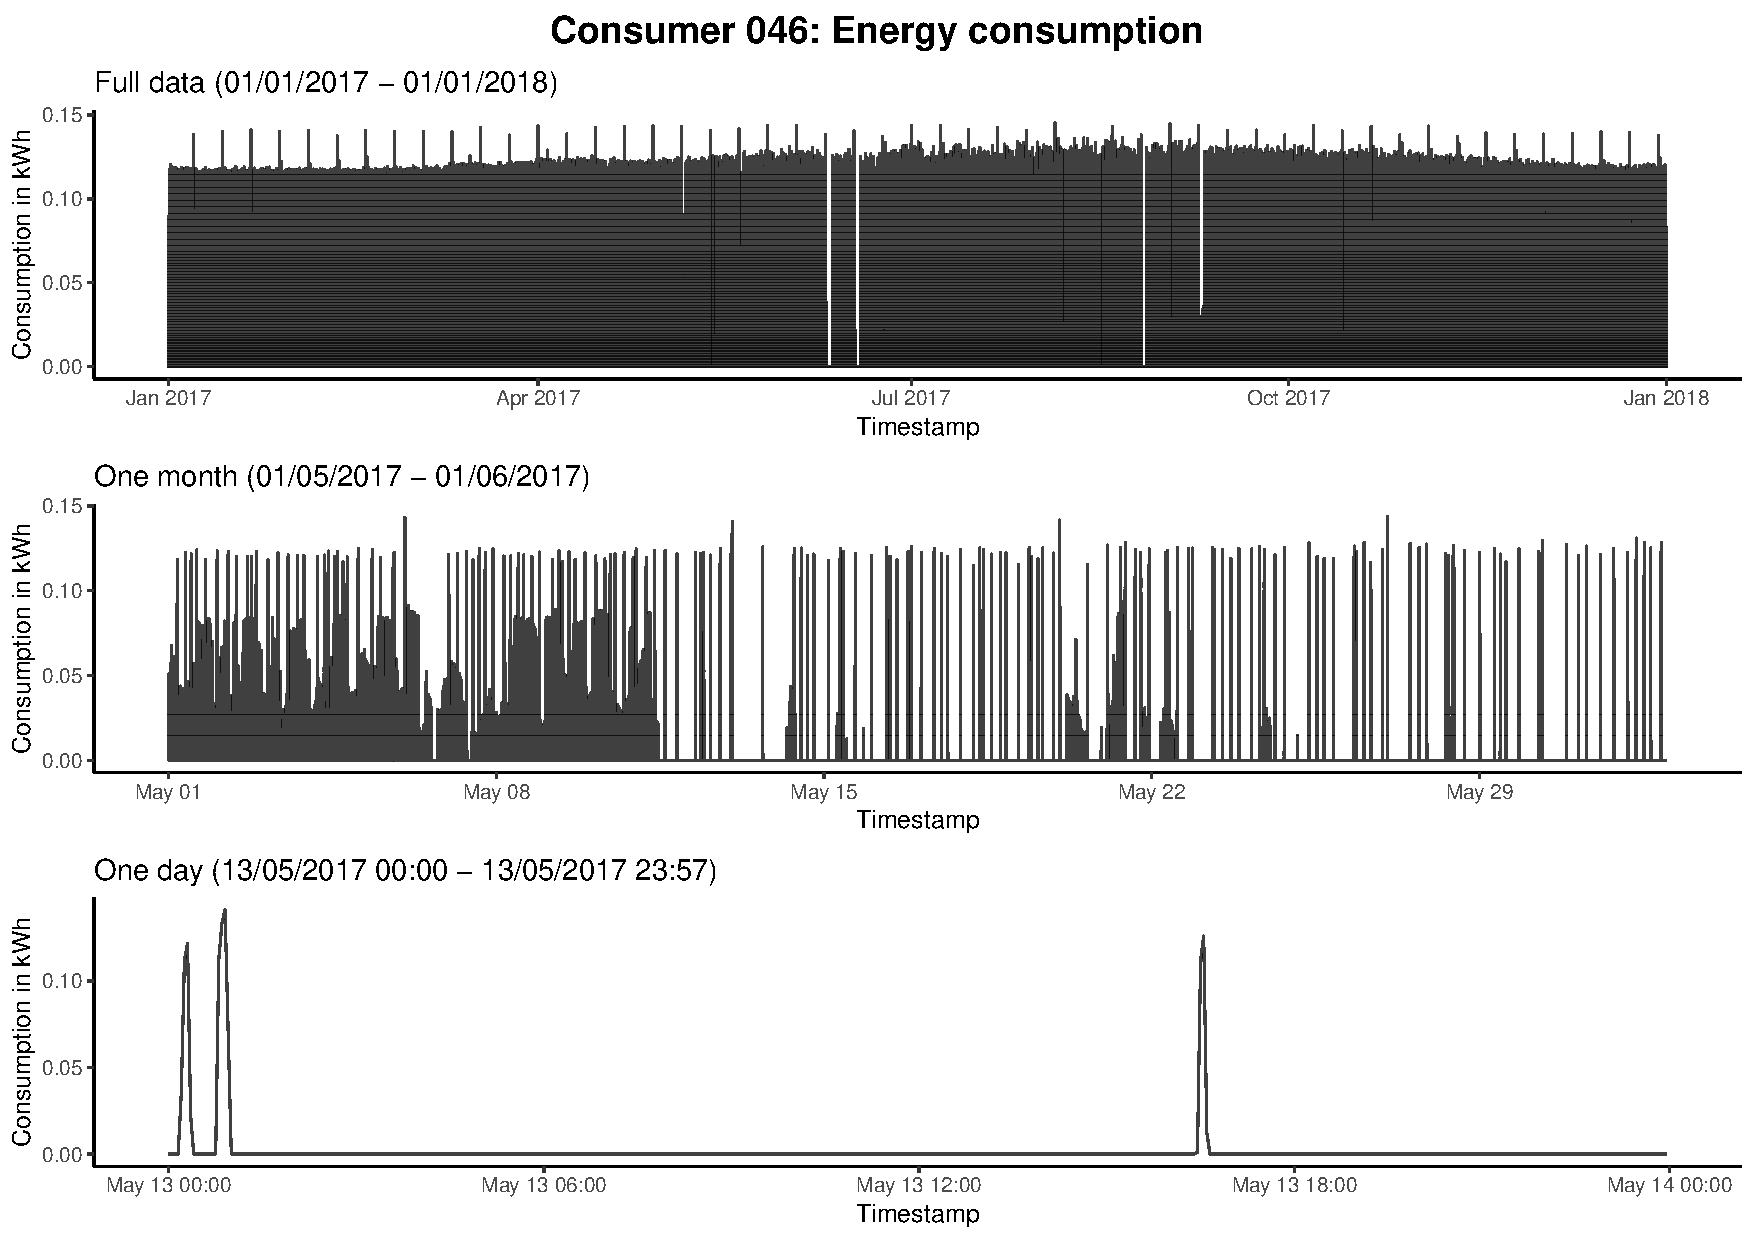
\includegraphics[width=\textwidth-0.85cm]{thesis/graphs/timeseries/c046_cons.pdf}
\end{figure}
\begin{figure}[!htbp]
        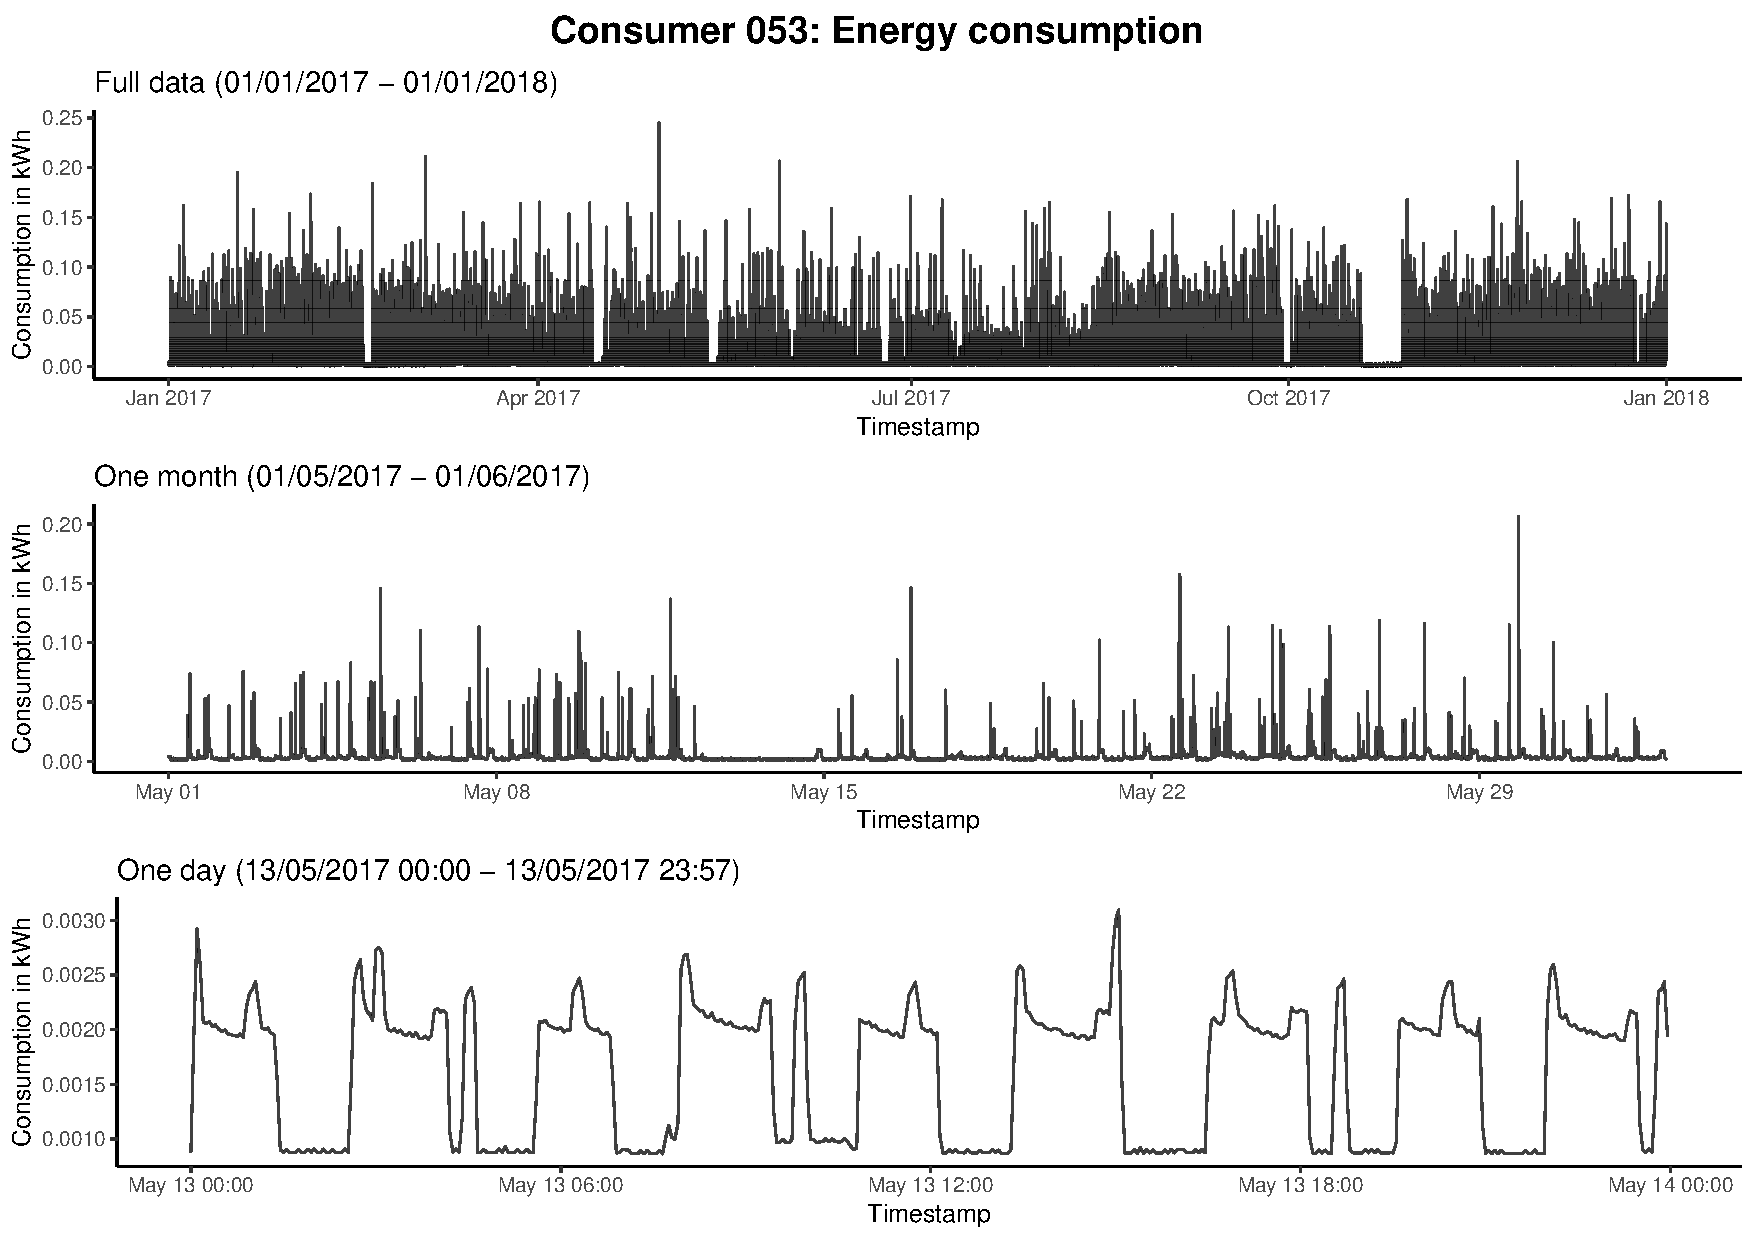
\includegraphics[width=\textwidth-0.85cm]{thesis/graphs/timeseries/c053_cons.pdf}\vspace{0.3cm}
        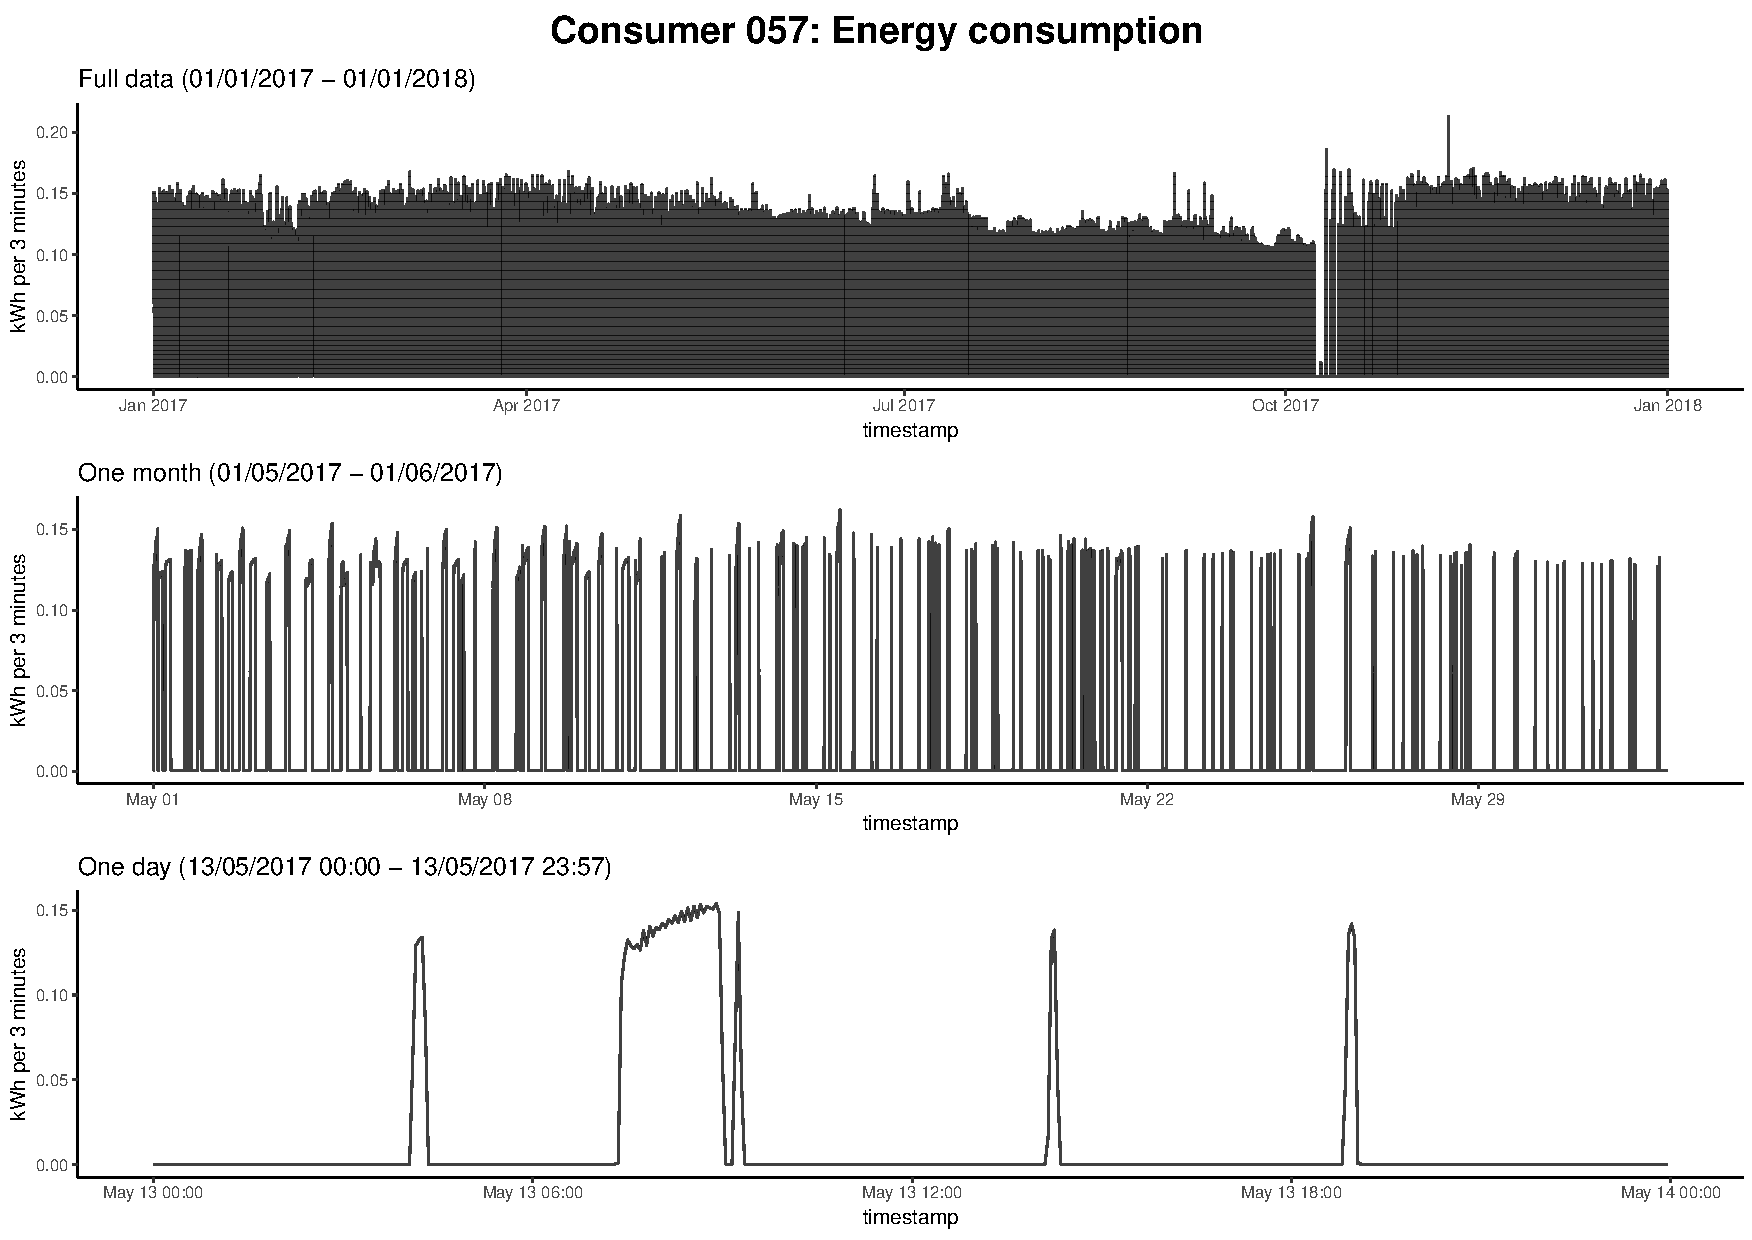
\includegraphics[width=\textwidth-0.85cm]{thesis/graphs/timeseries/c057_cons.pdf}
\end{figure}
\begin{figure}[!htbp]
        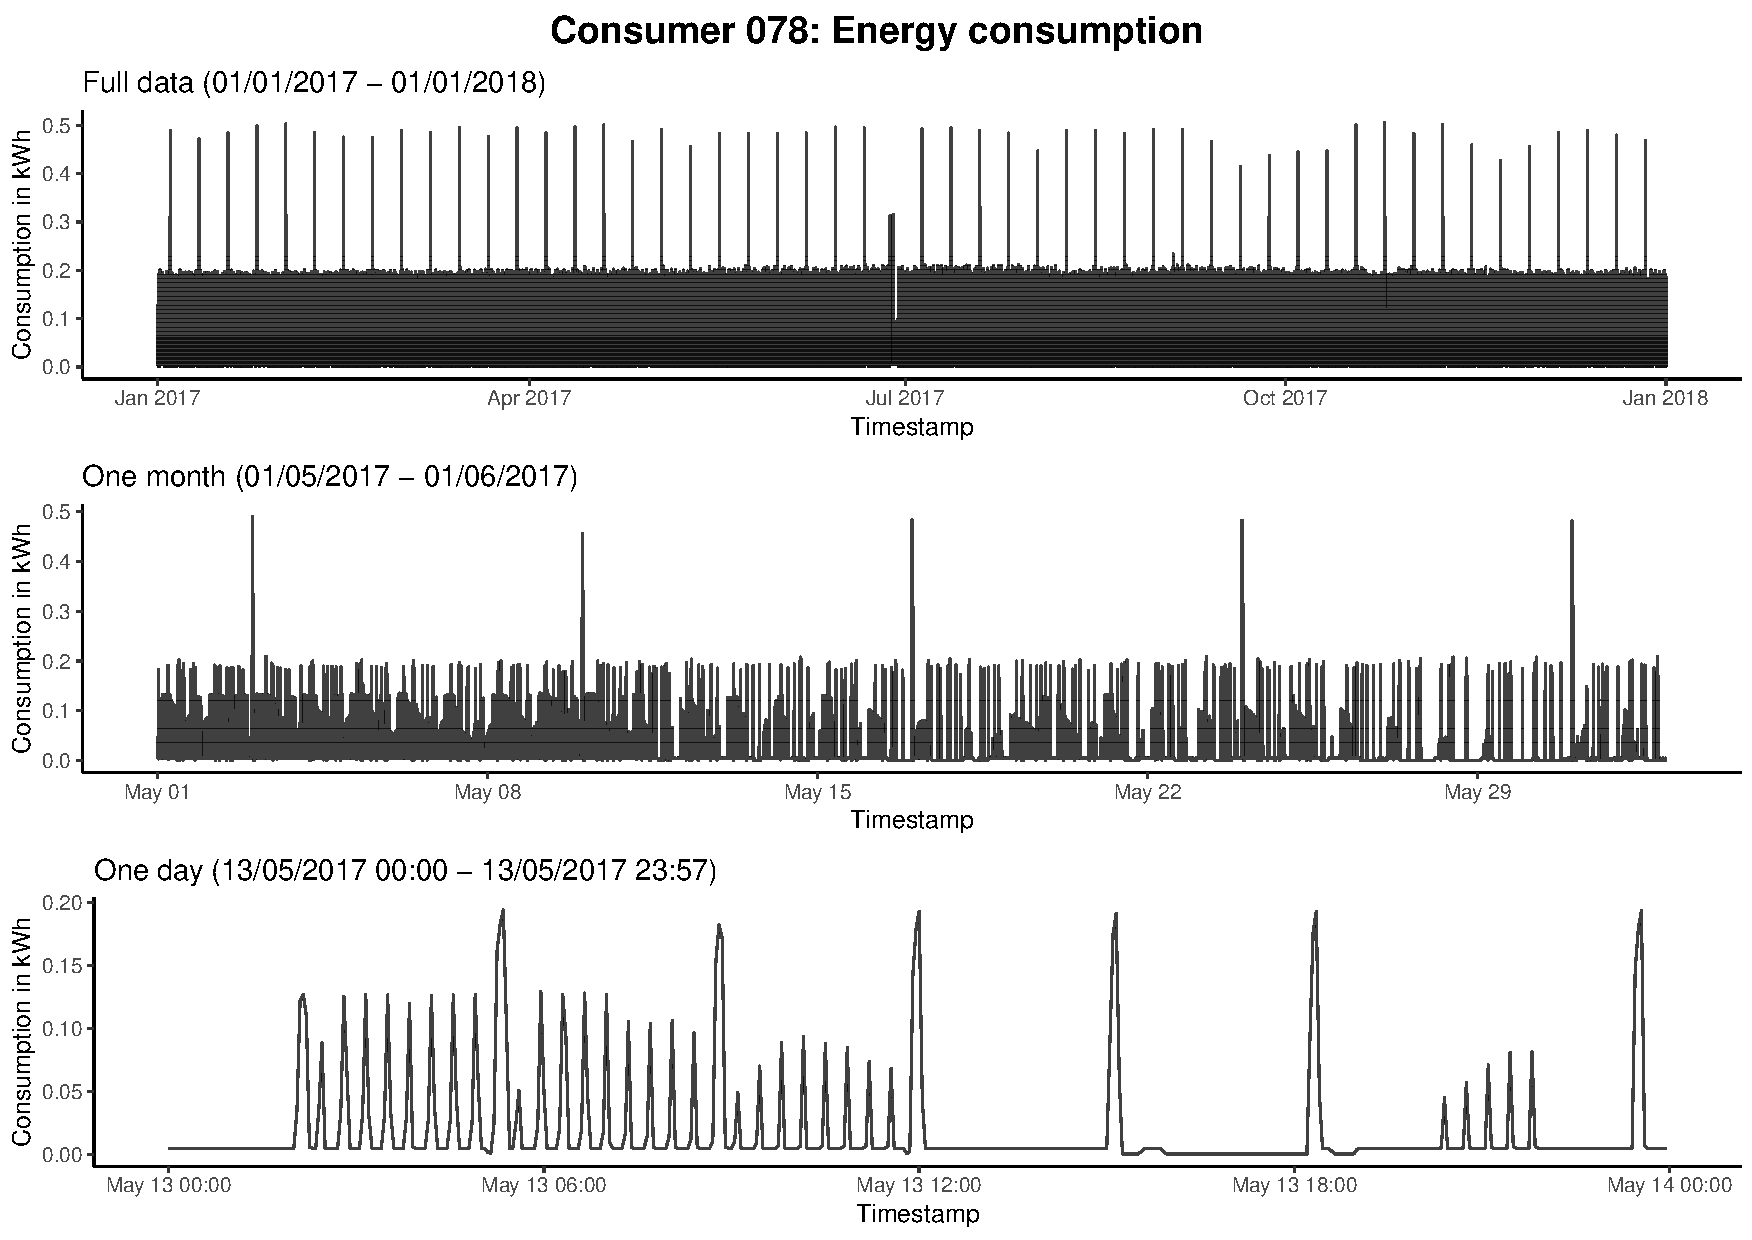
\includegraphics[width=\textwidth-0.85cm]{thesis/graphs/timeseries/c078_cons.pdf}\vspace{0.3cm}
        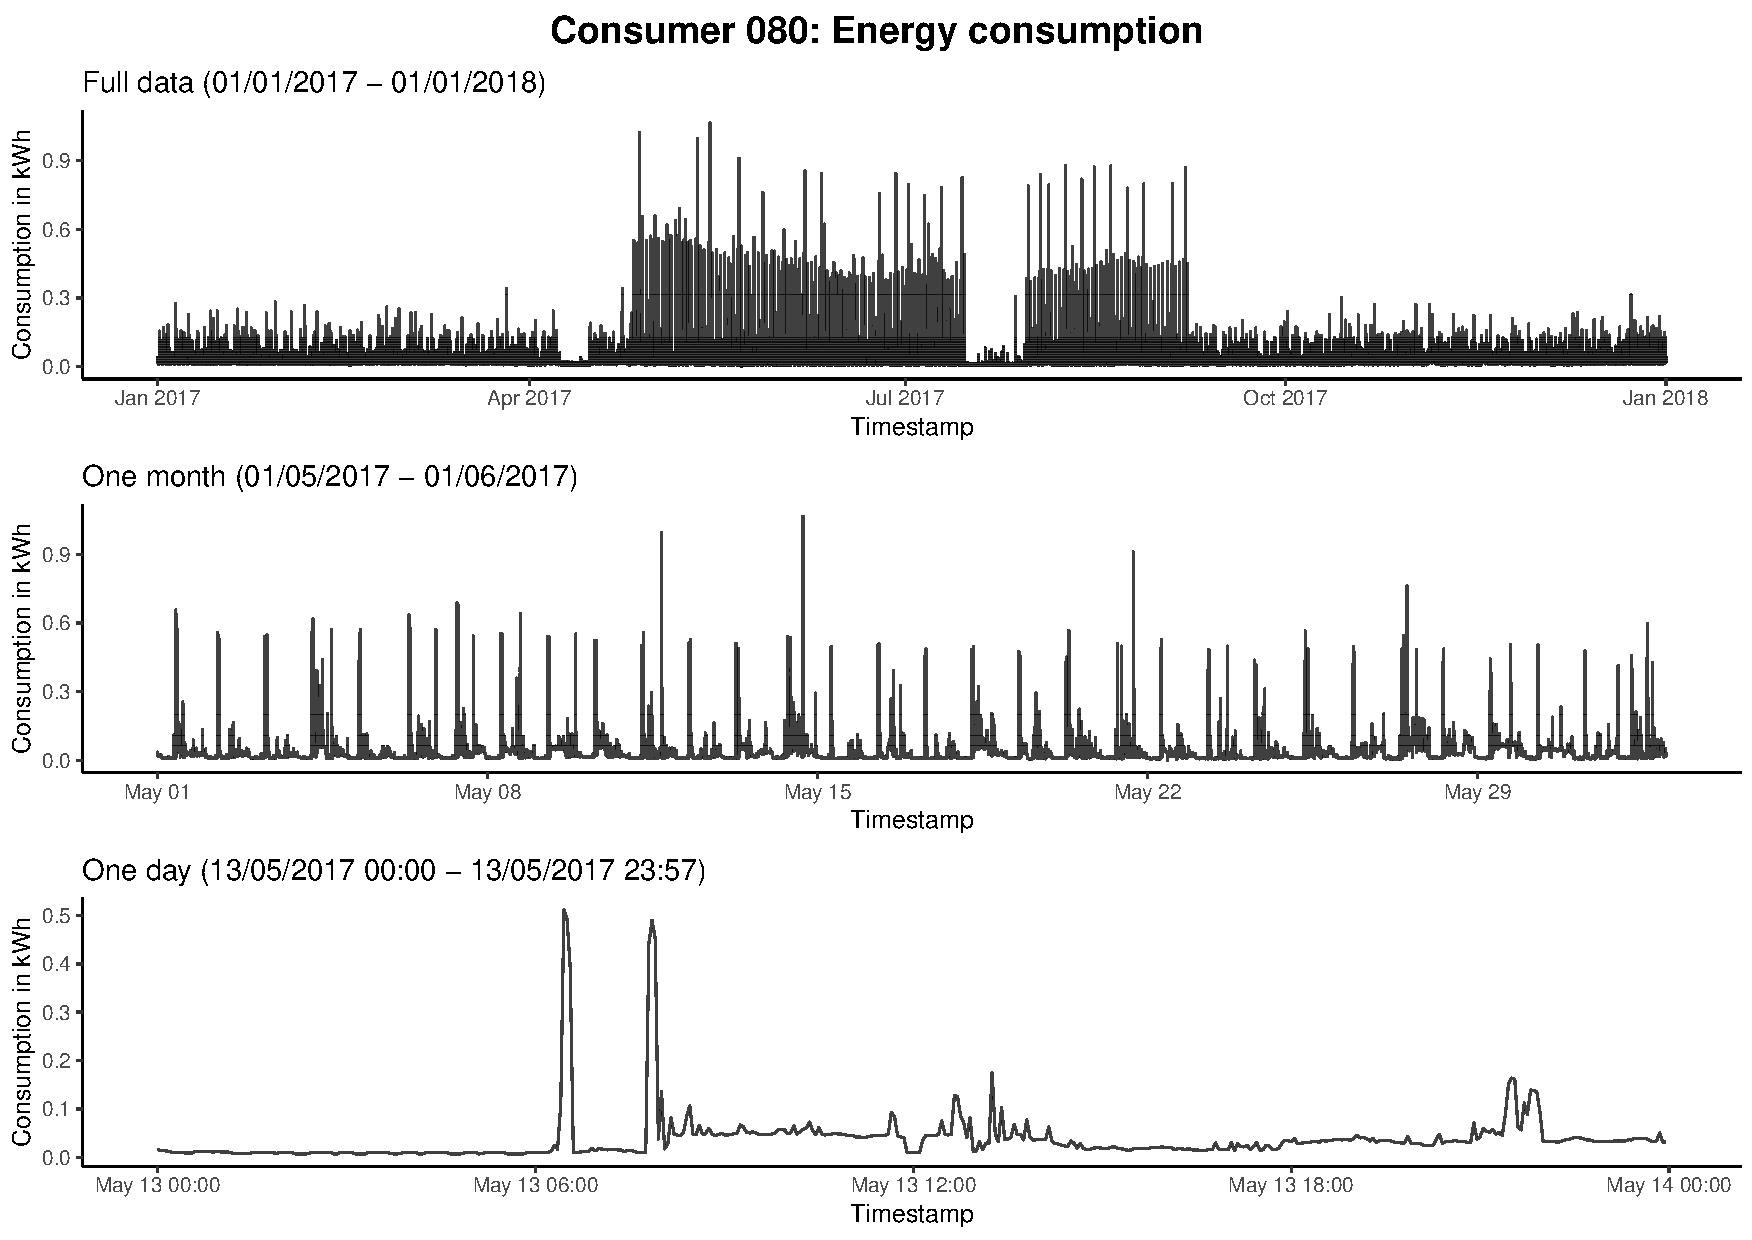
\includegraphics[width=\textwidth-0.85cm]{thesis/graphs/timeseries/c080_cons.pdf}
        \caption[Consumer data sets excluded due to peculiarities in the consumption patterns]{Consumer data sets excluded due to peculiarities in the consumption or production patterns. \quantnet\href{https://github.com/QuantLet/BLEM/tree/master/BLEMplotEnergyData}{BLEMplotEnergyData}}
\end{figure}
\end{centering}


\subsection*{\hypertarget{AppA2:Figures:Excludedp}{A2} Excluded prosumer data sets}\label{AppA2:Figures:Excludedp}

\begin{centering}
\begin{figure}[H]
        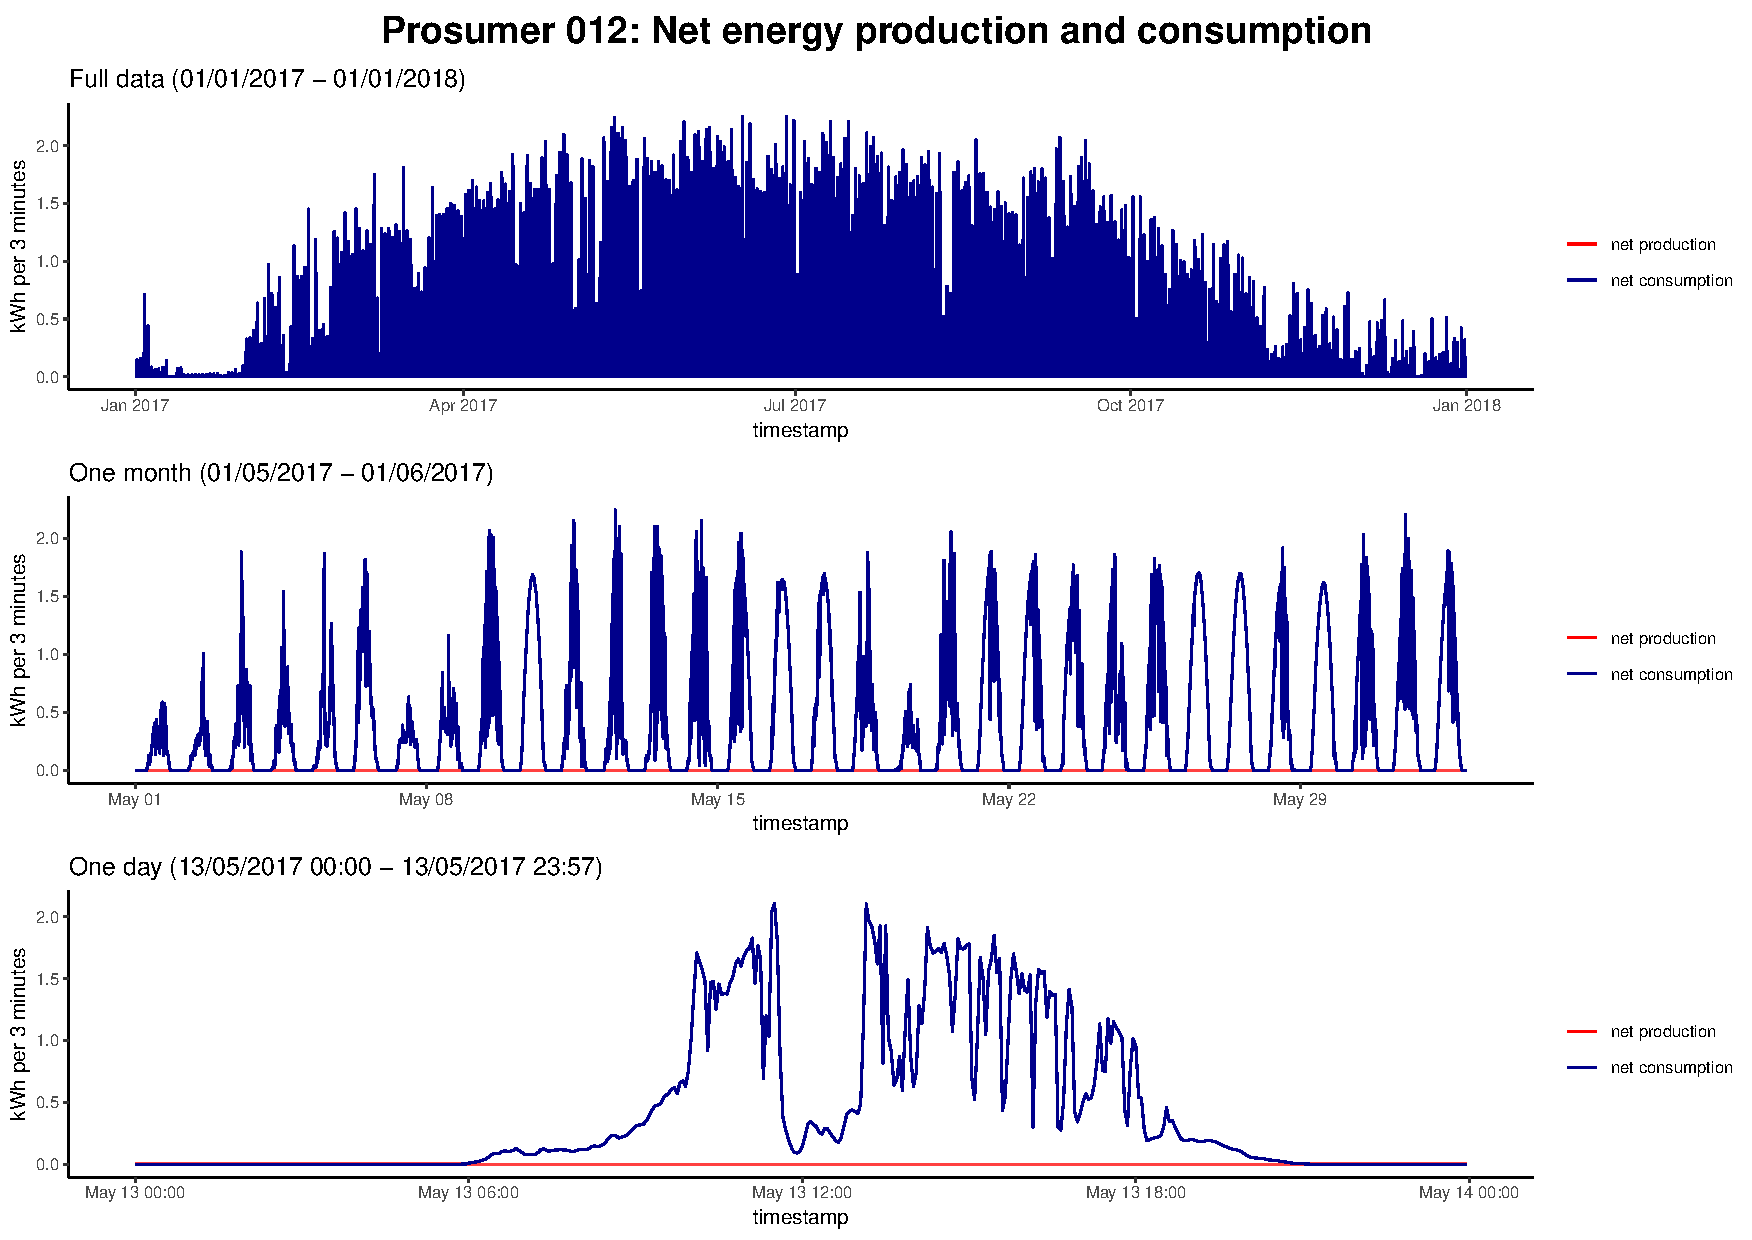
\includegraphics[width=\textwidth-0.85cm]{thesis/graphs/timeseries/p012_prod&cons.pdf}\vspace{0.3cm}
        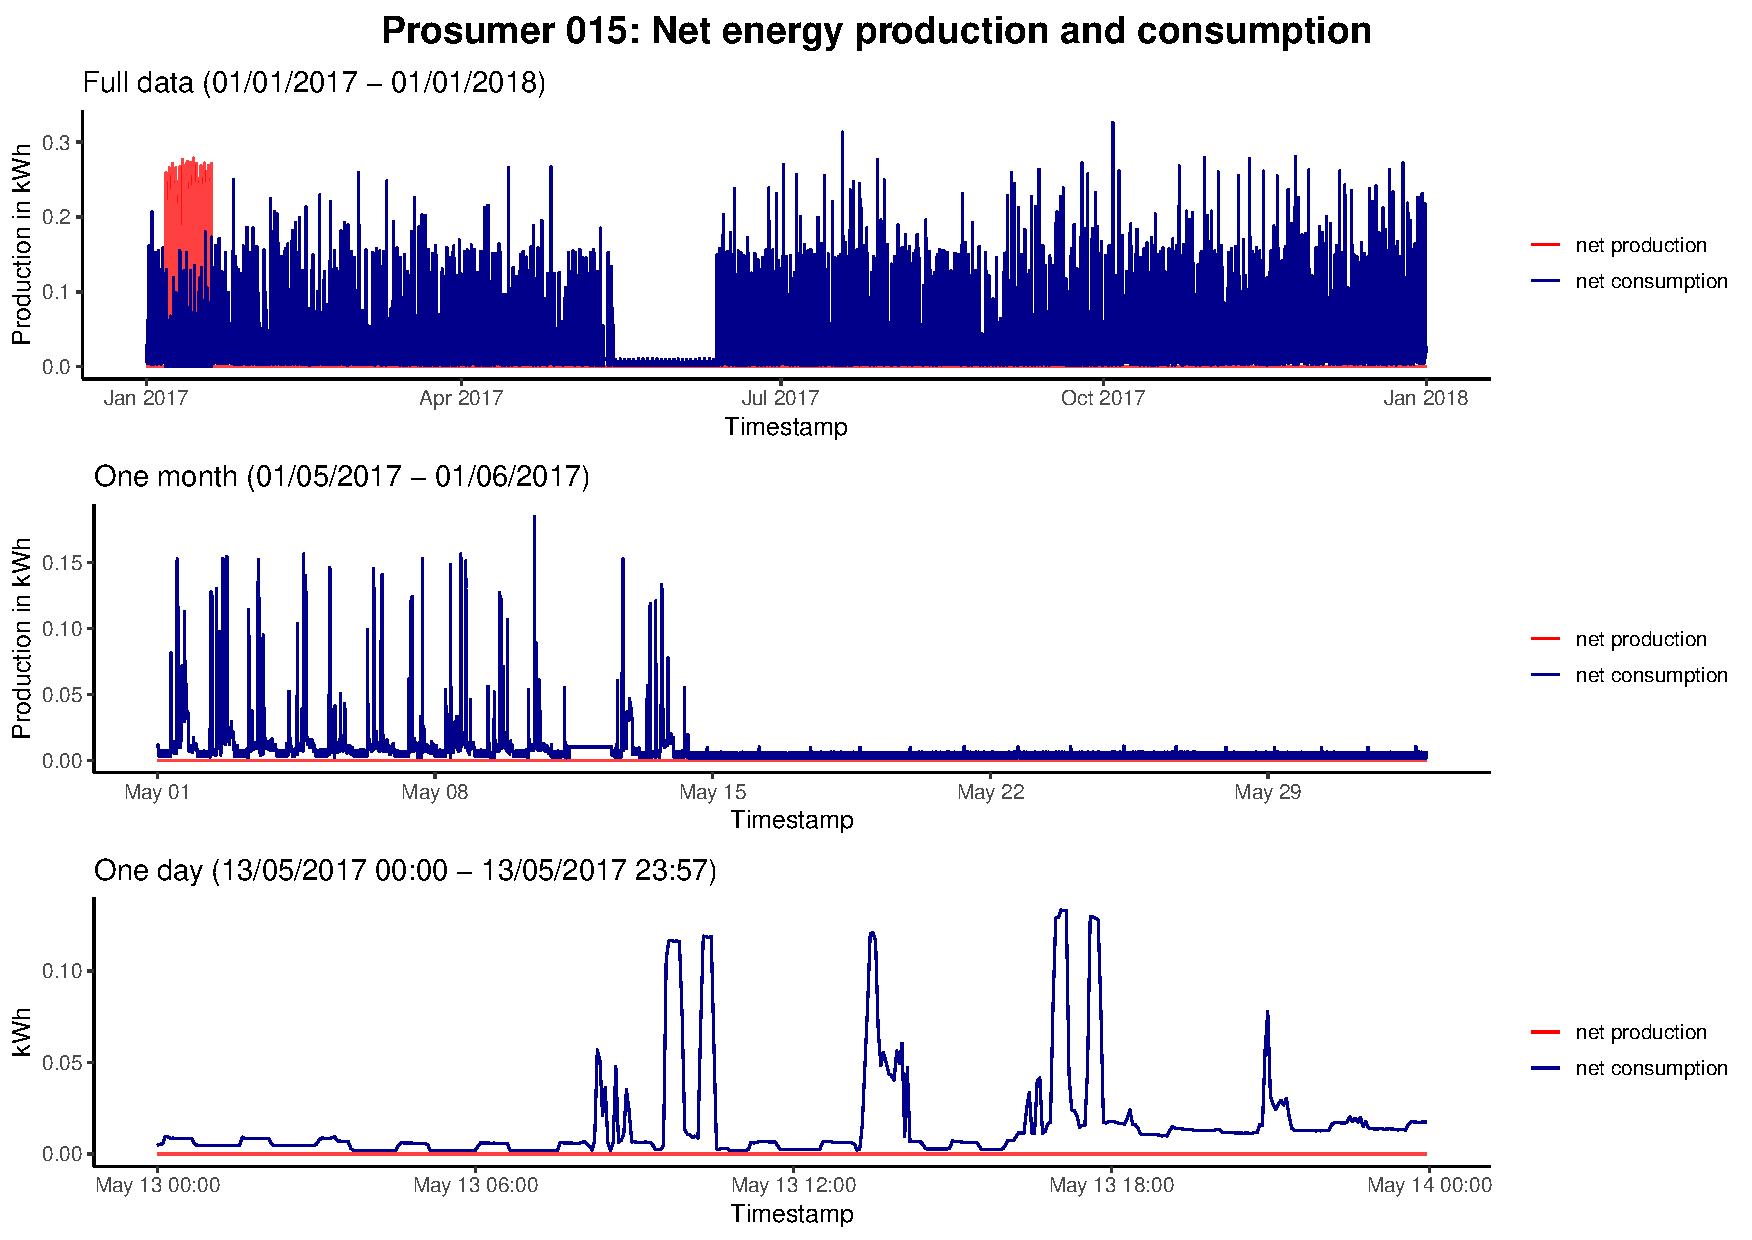
\includegraphics[width=\textwidth-0.85cm]{thesis/graphs/timeseries/p015_prod&cons.pdf}
        \caption[Prosumer data sets excluded due to peculiarities in the production patterns]{Prosumer data sets excluded due to peculiarities in the production patterns. \quantnet\href{https://github.com/QuantLet/BLEM/tree/master/BLEMplotEnergyData}{BLEMplotEnergyData}}
\end{figure}
\end{centering}


\subsection*{\hypertarget{AppA3:Figures:transform}{A3} Normalized log-consumption data}\label{AppA3:Figures:transform}

\begin{centering}
\begin{figure}[!htbp]
        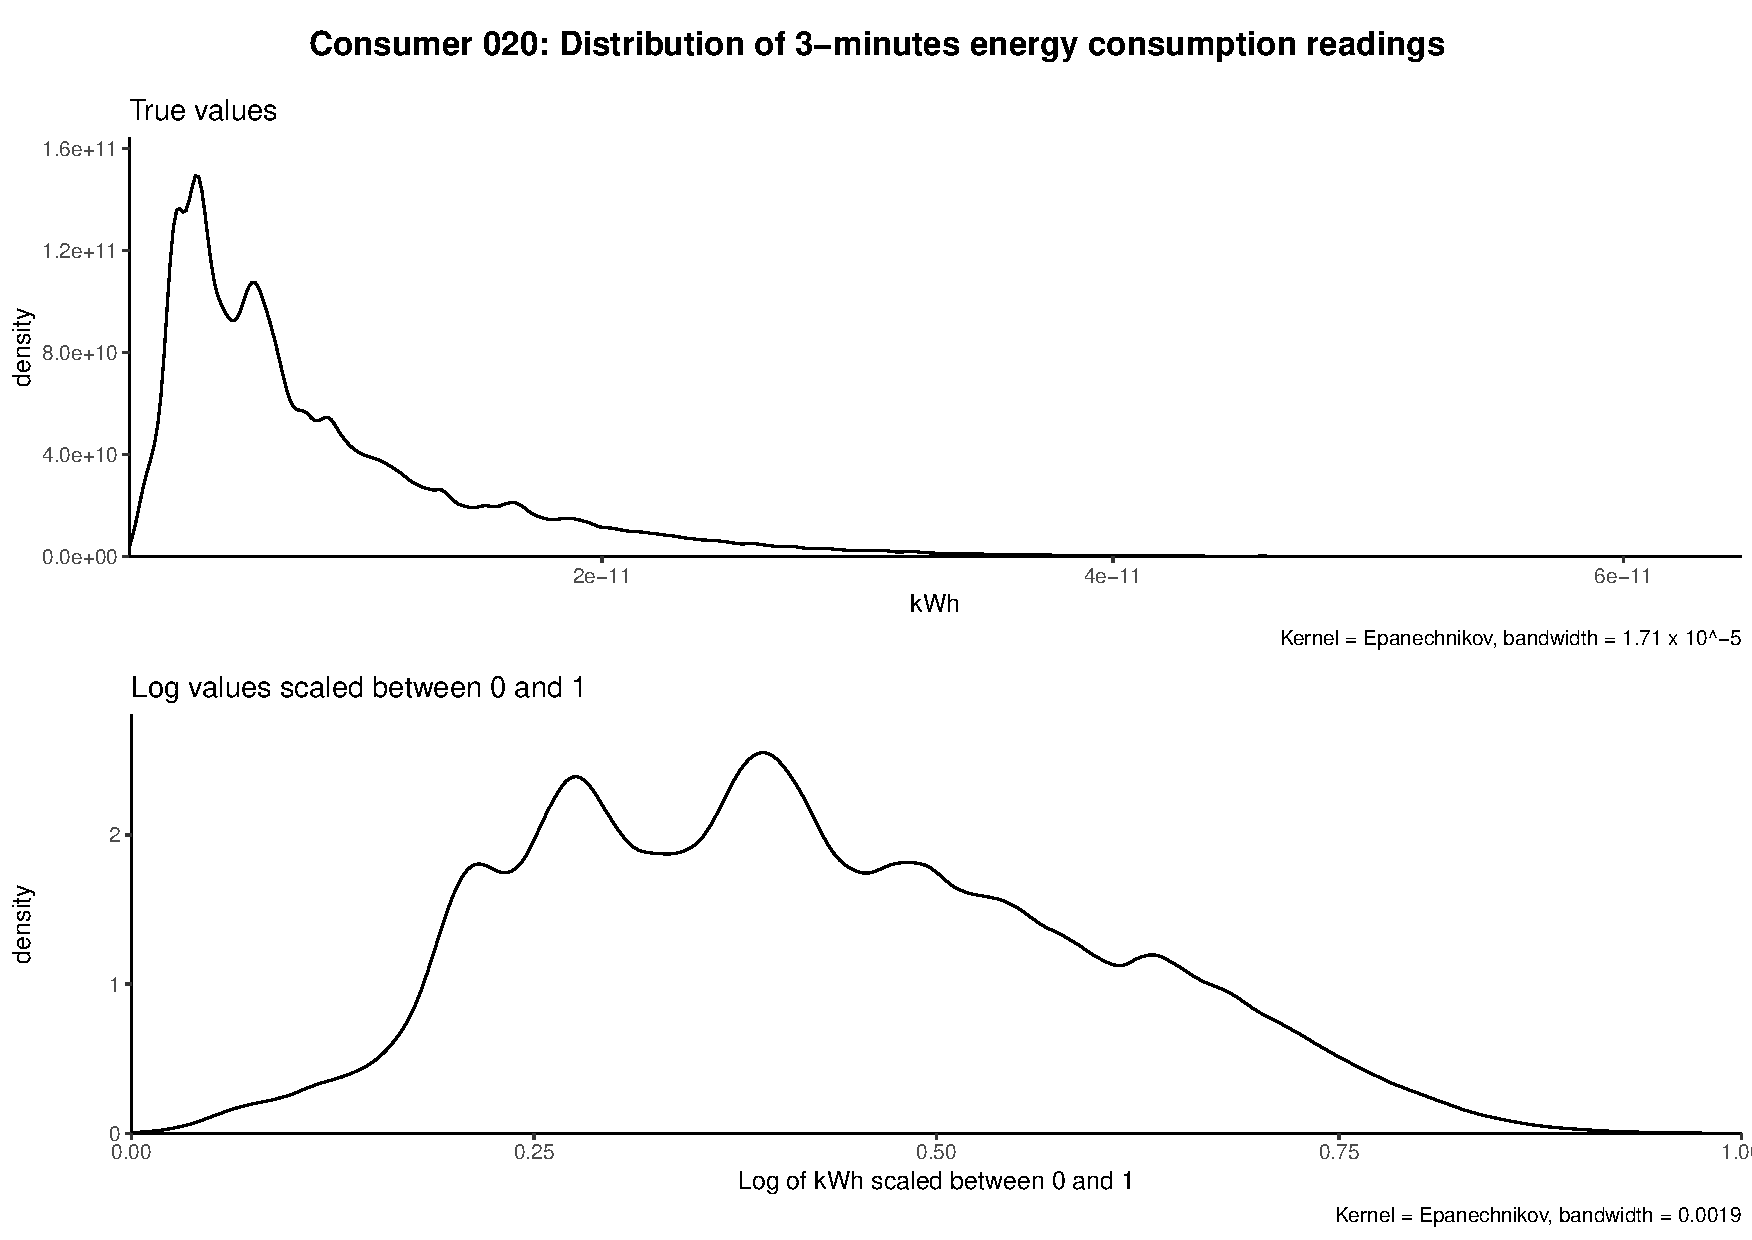
\includegraphics[width=\textwidth-0.85cm]{thesis/graphs/c020_density.pdf}
        \caption[Exemplary energy consumption distribution before and after transformation]{Consumer 020's density estimate of energy consumption values before and after transformation. \quantnet\href{https://github.com/QuantLet/BLEM/tree/master/BLEMplotScaling}{BLEMplotScaling}}
\end{figure}
\end{centering}


\subsection*{\hypertarget{AppA4:Figures:erroranalysis}{A4} Error analysis of consumer 027}\label{AppA4:Figures:erroranalysis}

\begin{centering}
\begin{figure}[H]
    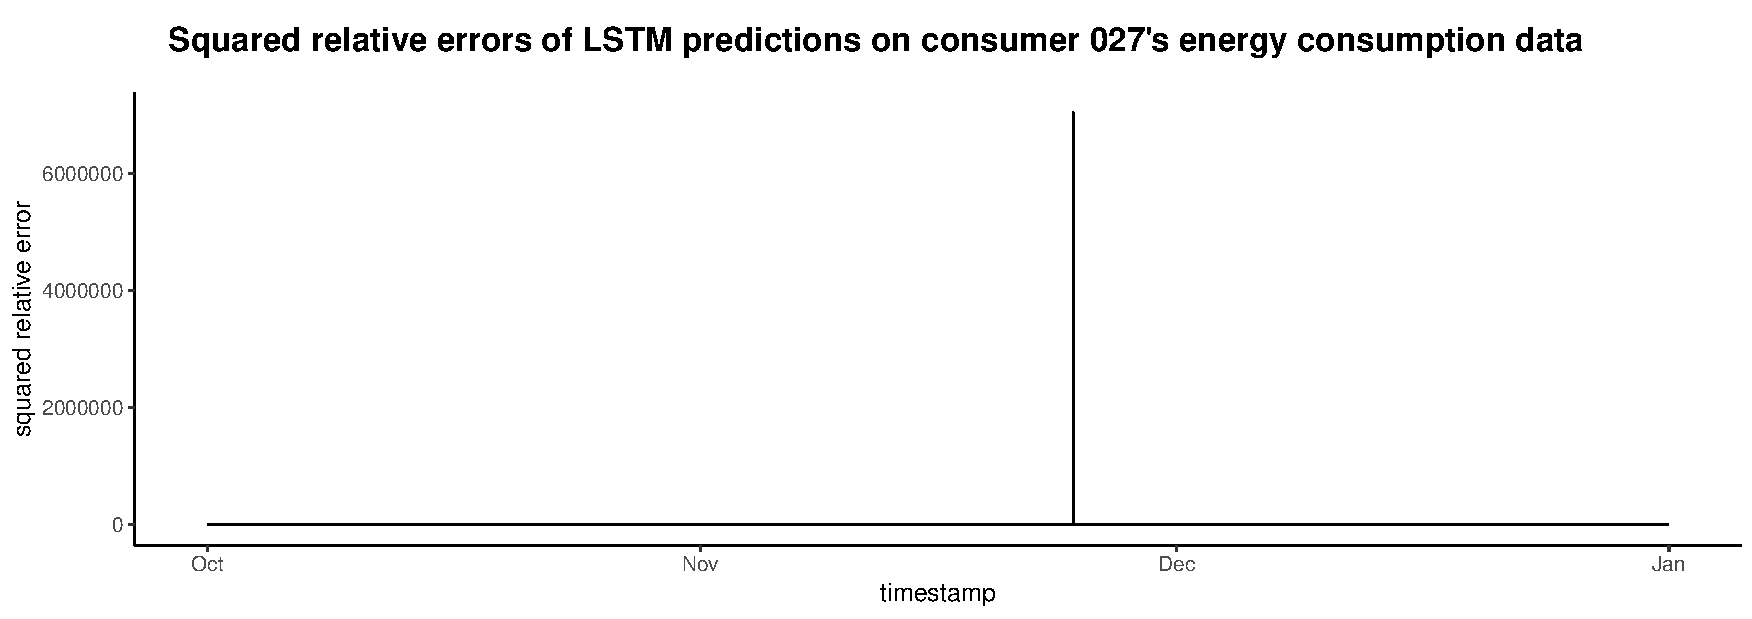
\includegraphics[width=\textwidth]{thesis/graphs/evaluation/c027_squarederrors.pdf}
    \caption[Squared relative errors of predictions by LSTM model on consumer 027]{Squared relative errors of predictions by LSTM model on data set of consumer 027. \quantnet\href{https://github.com/QuantLet/BLEM/tree/master/BLEMevaluateEnergyPreds}{BLEMevaluateEnergyPreds}}
\end{figure}
\end{centering}


\subsection*{\hypertarget{AppA5:Figures:heatmaps_p}{A5} Error evaluation of predictions on production data}\label{AppA5:Figures:heatmaps_p}

\begin{figure}[H]
    \centering
    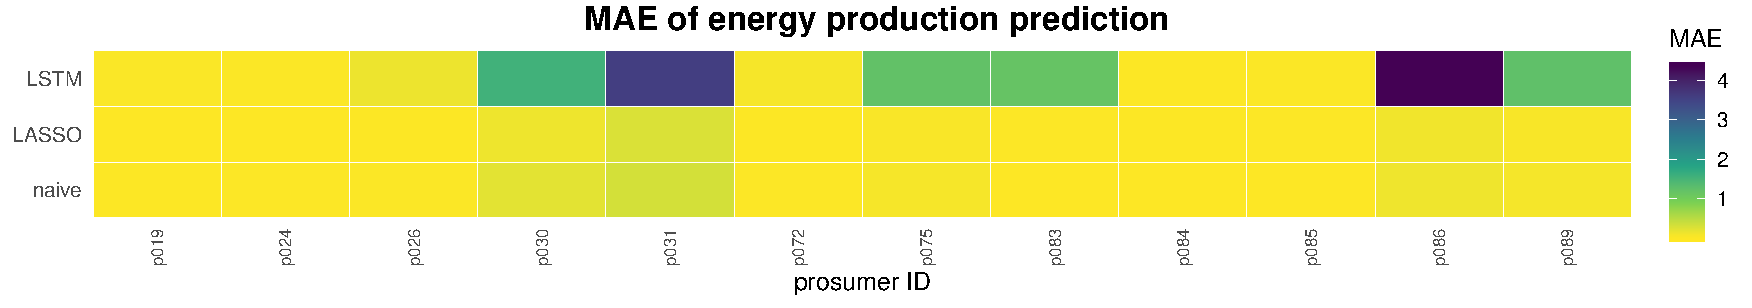
\includegraphics[width=\textwidth]{thesis/graphs/evaluation/p_heatmap_MAE.pdf}
    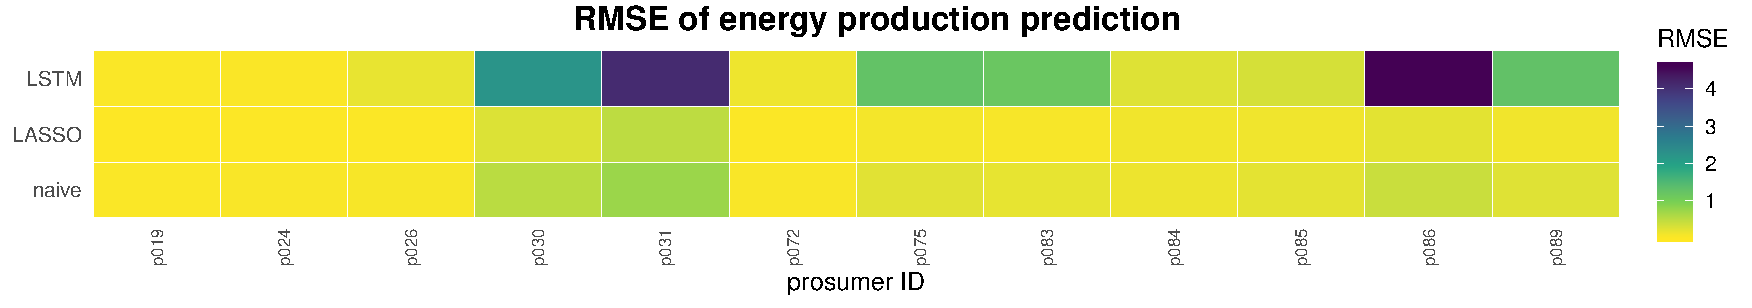
\includegraphics[width=\textwidth]{thesis/graphs/evaluation/p_heatmap_RMSE.pdf}
    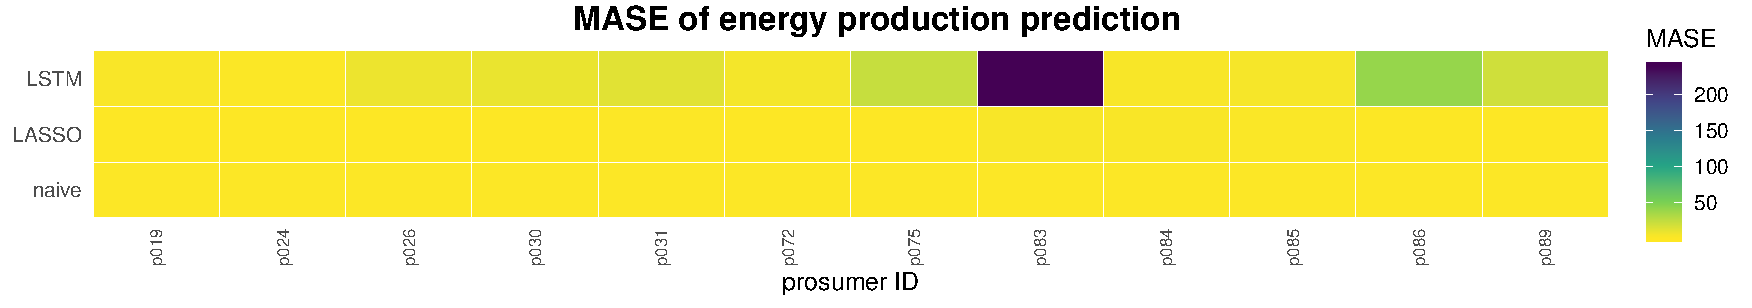
\includegraphics[width=\textwidth]{thesis/graphs/evaluation/p_heatmap_MASE.pdf}
    \caption[Heatmaps of error measures for production values]{Heatmaps of MAE, RMSE, and MASE scores for the prediction of production values per prosumer data set. \quantnet\href{https://github.com/QuantLet/BLEM/tree/master/BLEMevaluateEnergyPreds}{BLEMevaluateEnergyPreds}}
\end{figure}


\subsection*{\hypertarget{AppA6:Figures:producer_all}{A6} Overview of prosumers' energy production time series}\label{AppA6:Figures:producer_all}

\begin{figure}[H]
    \centering
    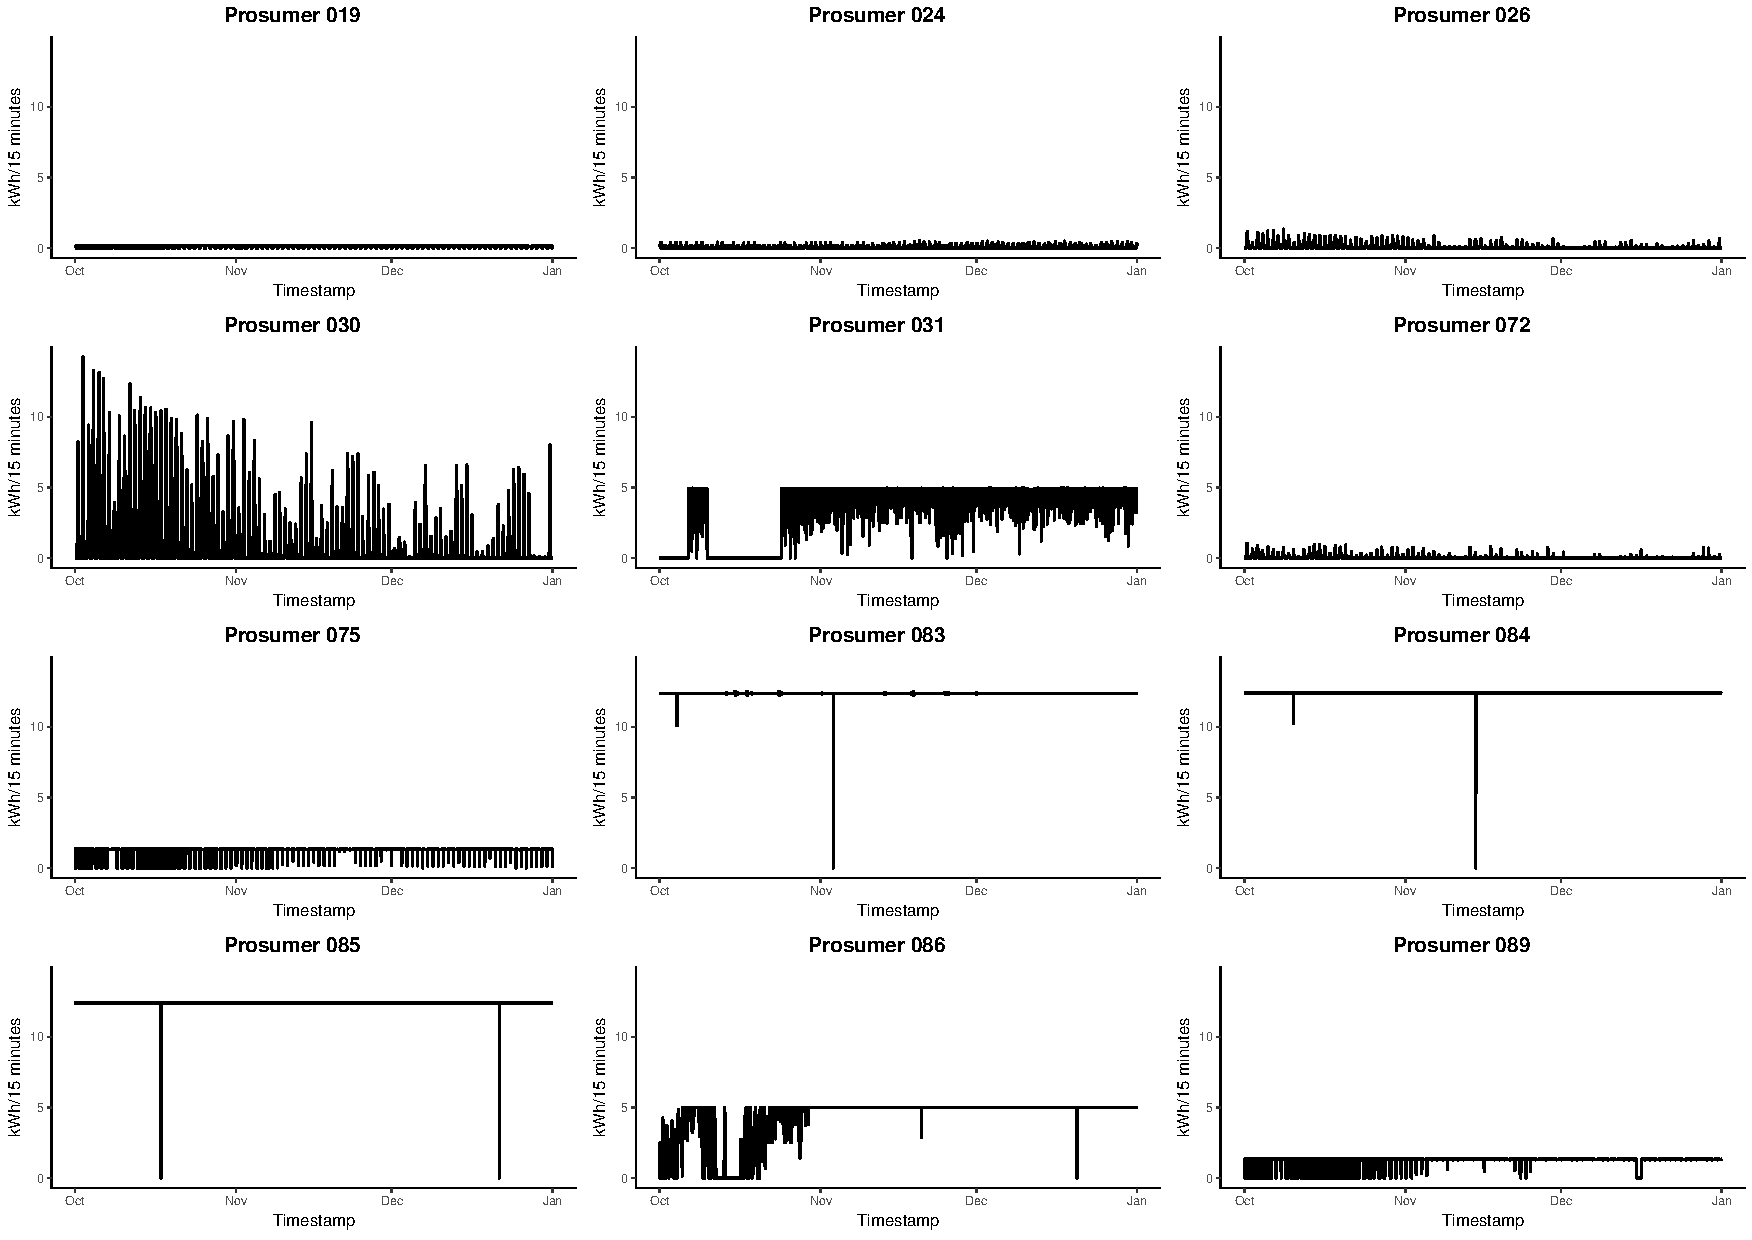
\includegraphics[width=\textwidth]{thesis/graphs/marketsimulation/producers_all.pdf}
    \caption[Energy production time series of prosumers relevant for market simulation]{Energy production time series of prosumer data sets that are potentially relevant for the market simulation in the time period from 01.10.2017 00:00 to 01.01.2018 00:00. \quantnet\href{https://github.com/QuantLet/BLEM/tree/master/BLEMmarketSimulation}{BLEMmarketSimulation}}
\end{figure}


\newpage
\subsection*{\hypertarget{AppA7:Figures:marketsimulation_pred}{A7} Market simulation with predicted values}\label{AppA7:Figures:marketsimulation_pred}

\begin{figure}[H]
    \centering
    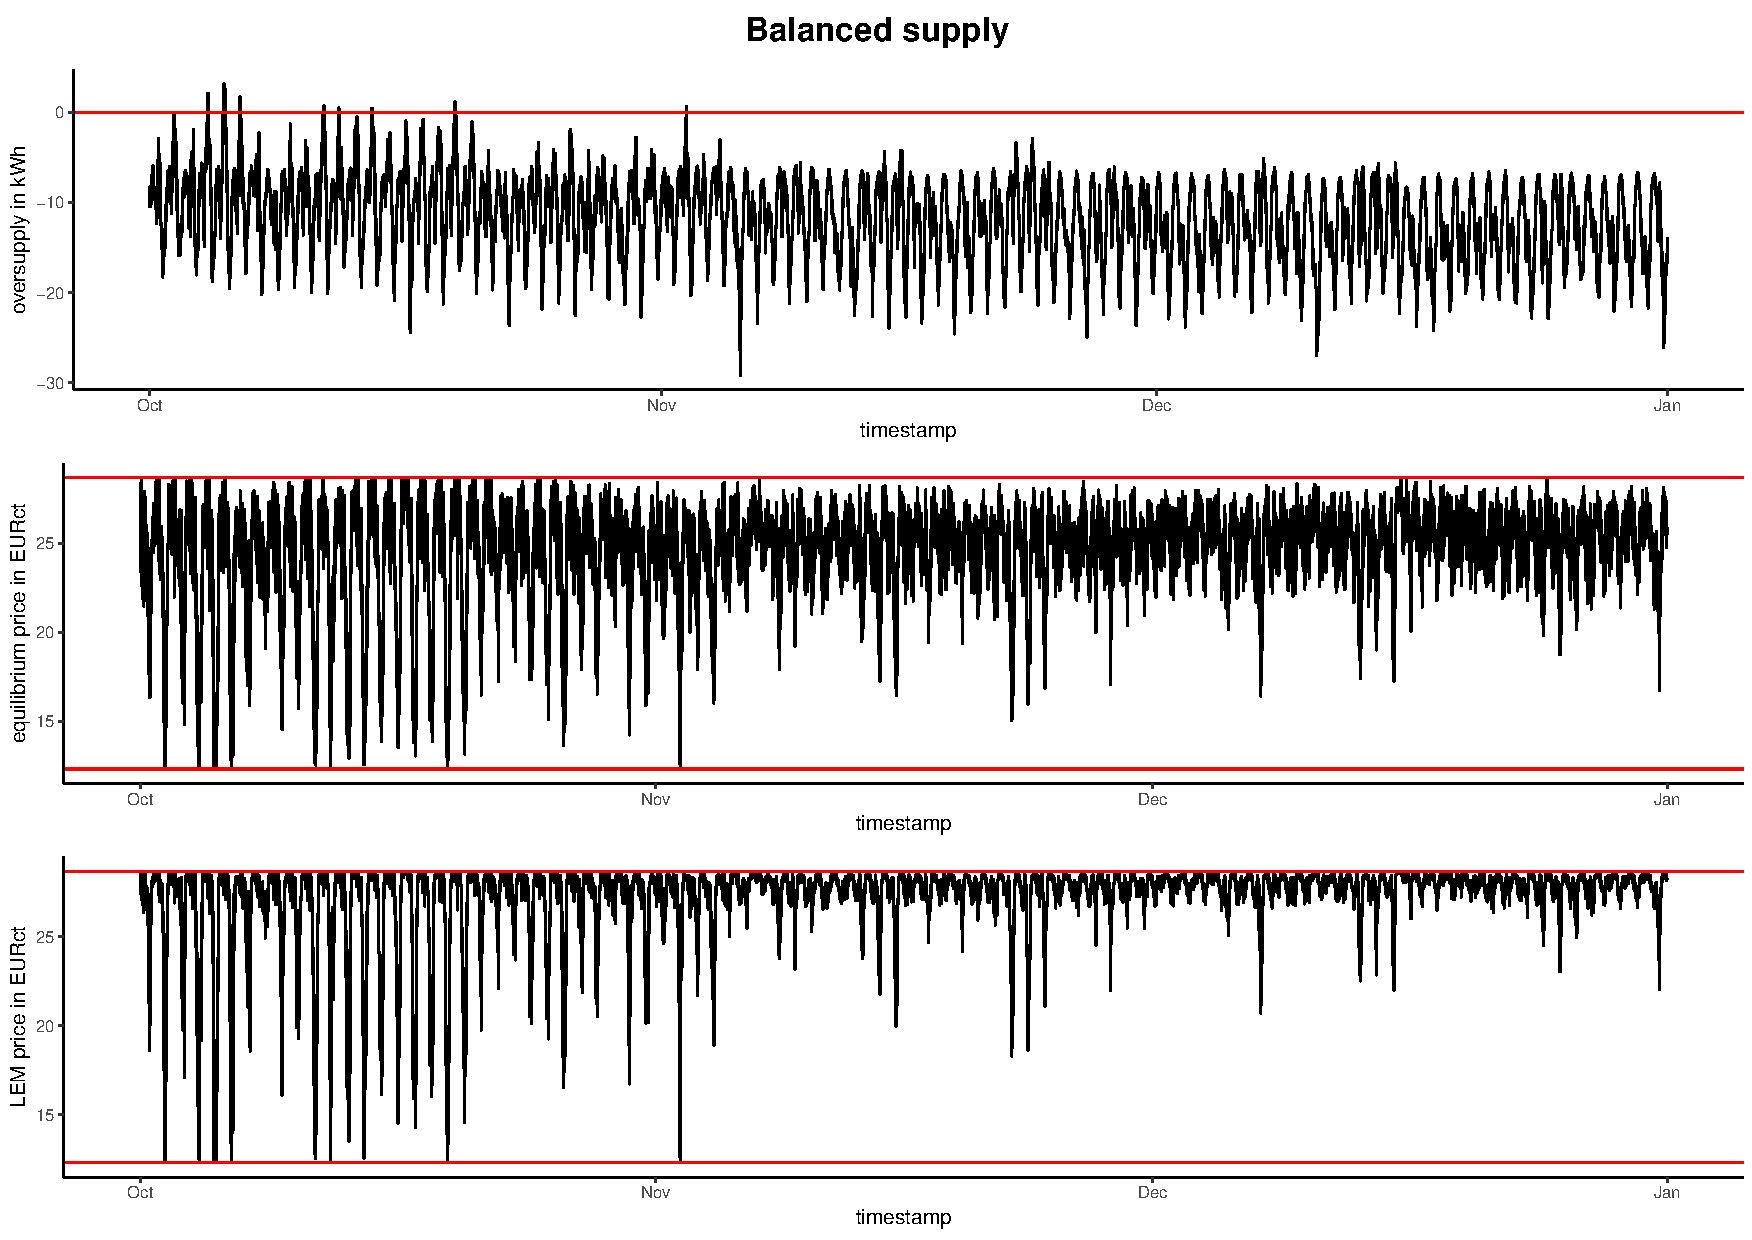
\includegraphics[width=\textwidth-.85cm]{thesis/graphs/marketsimulation/marketoutcome_pred_balanced.pdf}\\\vspace{.6cm}
    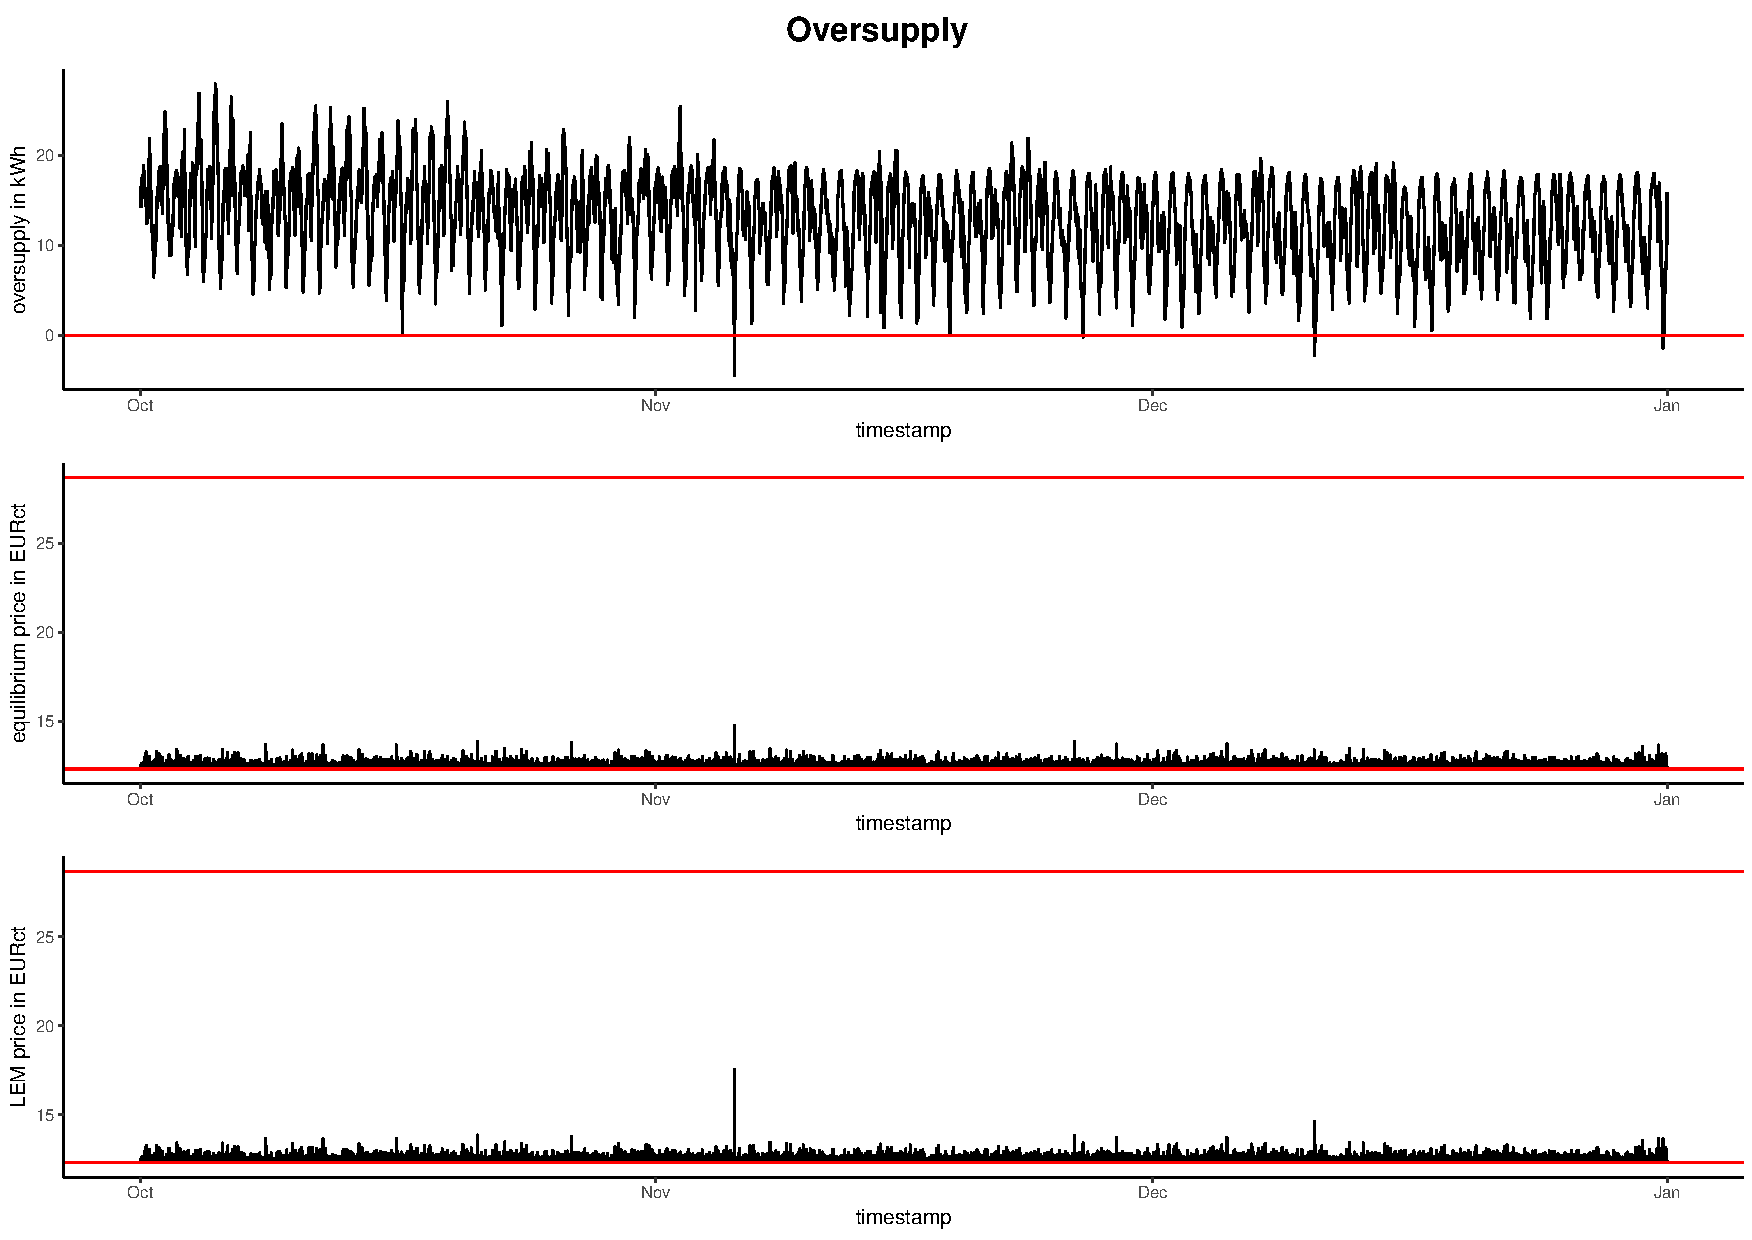
\includegraphics[width=\textwidth-.85cm]{thesis/graphs/marketsimulation/marketoutcome_pred_oversupply.pdf}
\end{figure}
    
\begin{figure}[H]
    \centering
    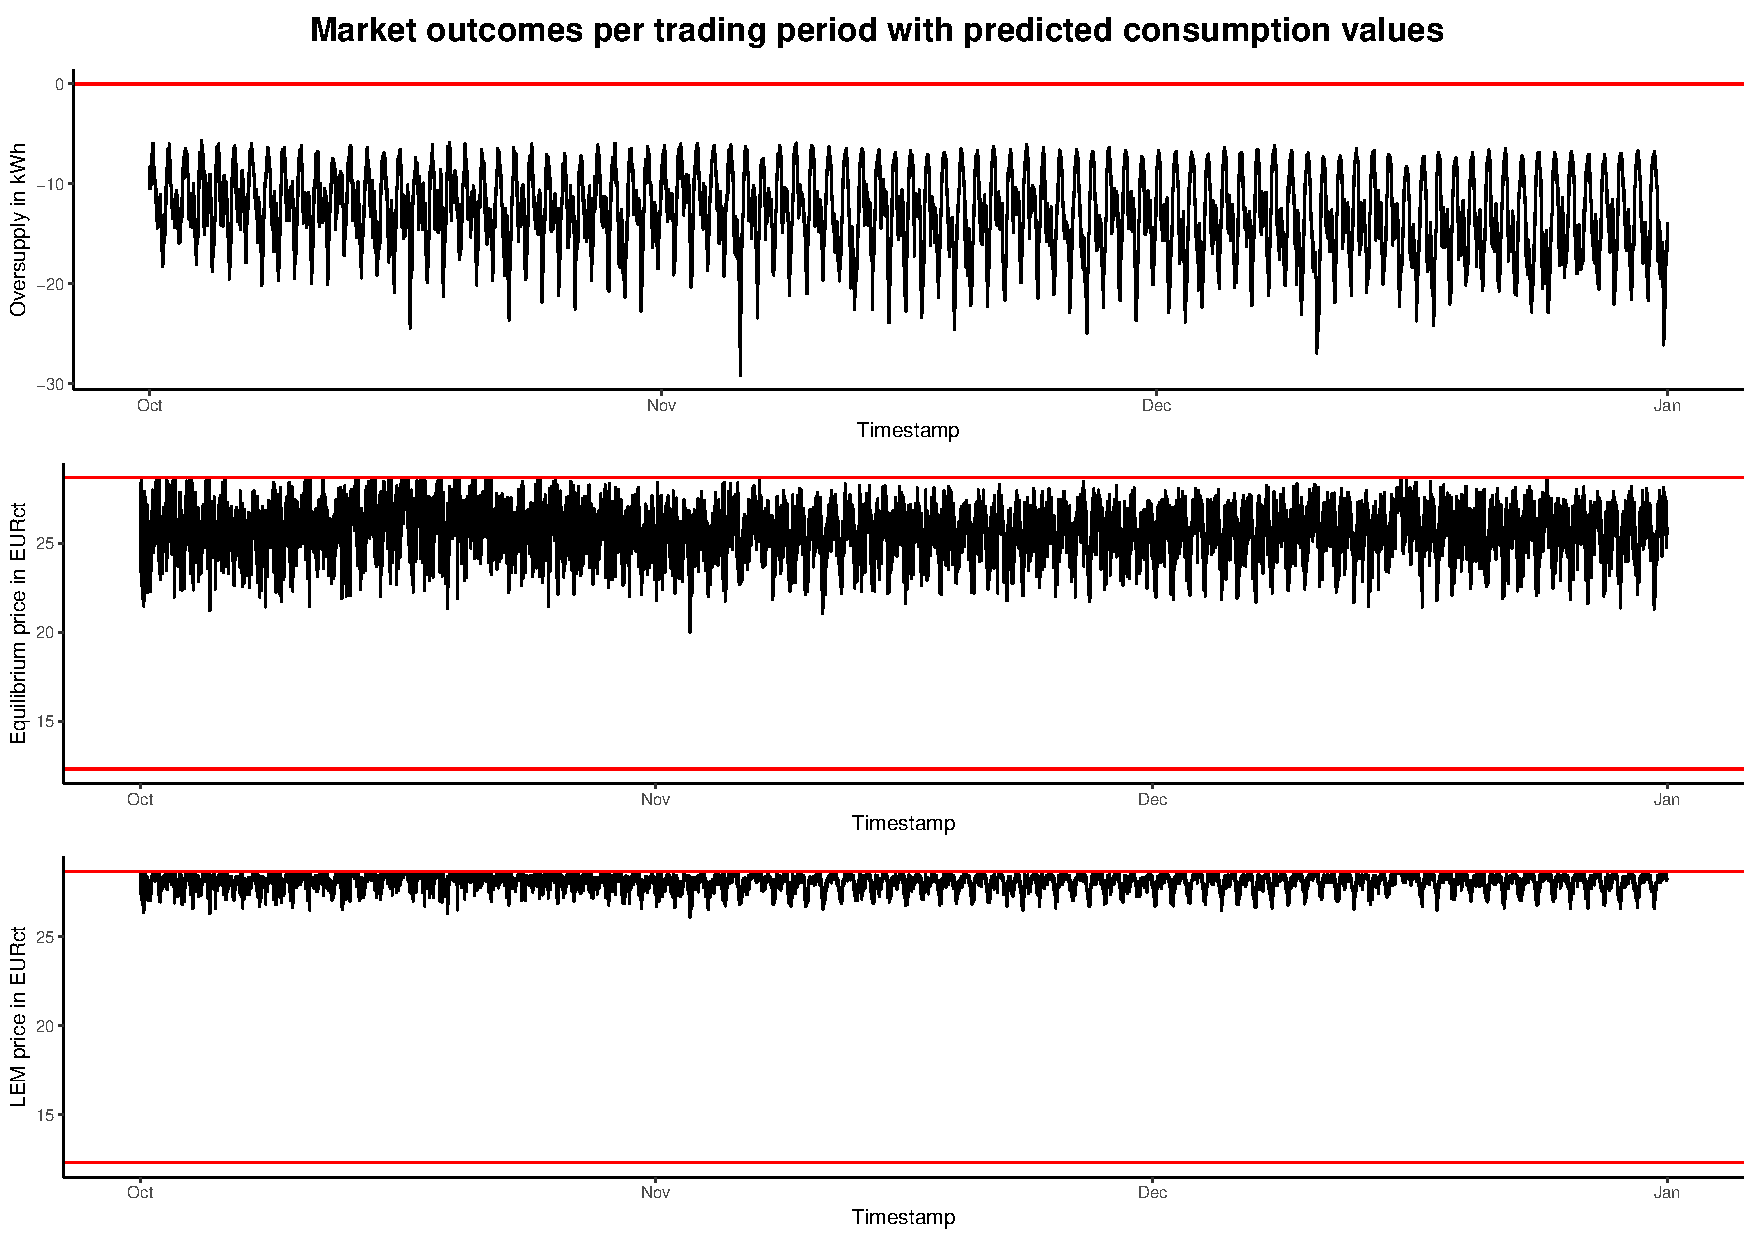
\includegraphics[width=\textwidth-.85cm]{thesis/graphs/marketsimulation/marketoutcome_pred_undersupply.pdf}
    \caption[Market outcomes simulated in three supply scenarios with predicted values]{Market outcomes per trading period simulated with predicted values in a balanced, an oversupply, and an undersupply scenario. \quantnet\href{https://github.com/QuantLet/BLEM/tree/master/BLEMmarketSimulation}{BLEMmarketSimulation}}
\end{figure}

%%%%%%%%%%%%%%%%%%%%%%%%%%%%%%%%%%%%%%%%%%%%%%%%%%%%%%%%%%%%
